\section{GPU Vs CPU}

从这两张图（图1.1）来看，左侧代表中央处理器（CPU），右侧代表图形处理器（GPU）。两者似乎都包含相似
的组件或单元。例如，两者都有动态随机存取存储器（DRAM）和不同级别的缓存。具体来说，GPU配备了两个缓存级别，其功能与
CPU中的缓存类似；而CPU包含三个缓存级别——L1、L2和L3。接下来来看算术逻辑单元（ALU）。

这个单元负责执行应用程序的指令。CPU中只有数量有限的ALU，而GPU则包含数百甚至数千个类似单元，称为核心（Core）。鉴
于以上相似性——两者都有全局内存、都有多级缓存——我们自然会问：它们之间到底有什么区别？


\begin{figure}
    \centering
    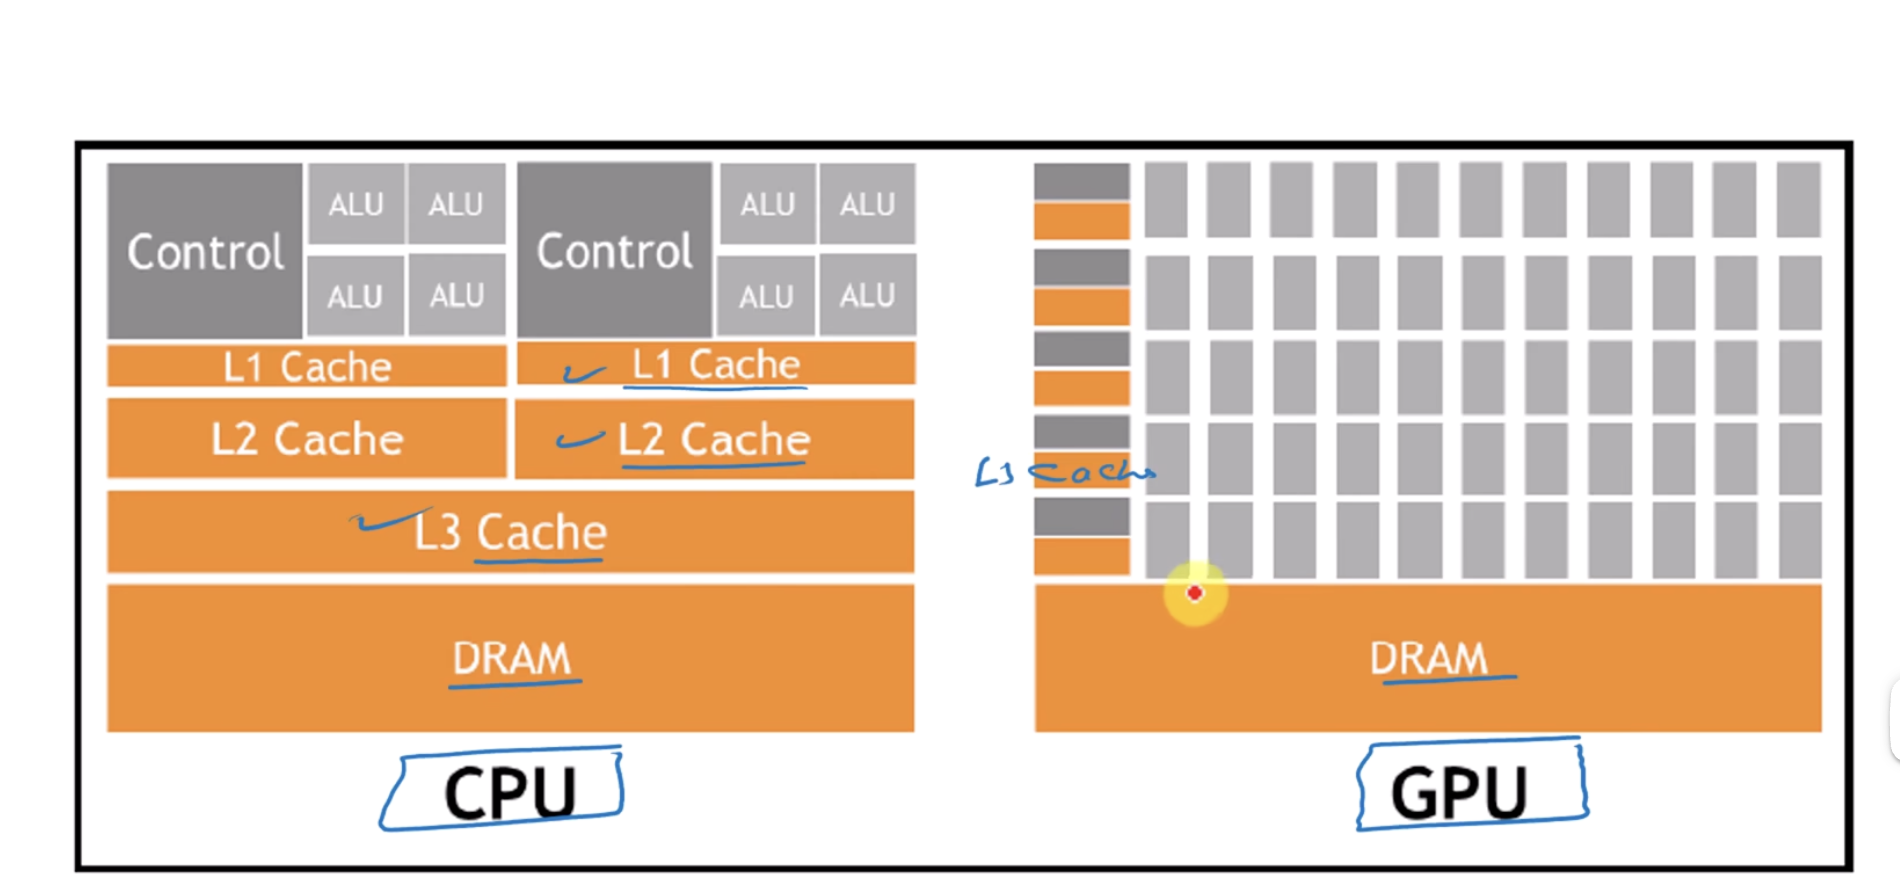
\includegraphics[width=0.8\linewidth]{resources/cuda-001.png}
    \caption{GPU Vs CPU}
    \label{fig:placeholder}
\end{figure}


\subsection{ALU与核心的对比}

CPU中有ALU，而GPU中有核心。为了理解它们的区别，以及为什么大多数系统同时需要CPU和GPU，让我们来仔细分析。在一对一
的比较中，CPU中的ALU明显比GPU中的核心更强大、更复杂。这里的"一对一"指将CPU中的一个ALU与GPU中的一个核心进行
单独对比。当我们说一个ALU"更强大"时，指的是速度等属性——例如现代CPU的运行频率可达3到4 GHz。而作为对比，一款
2020年发布的GPU——英伟达A100——其频率范围在765到1200 MHz之间。


需要明确的是，1200 MHz 意味着 1.2 GHz，大约只是主流 CPU 速度的四分之一。另一方面，GPU 核心更为专精，通常设计用于
高效执行特定类型的任务。CPU 中的 ALU 是为通用任务设计的，专注于快速执行单个线程。而 GPU 核心则是为并行性设计的——
它们经过优化，可以同时处理大量线程，这使它们非常适合像渲染图形这类需要对大量元素并行执行相同操作的任务。

理解 CPU 和 GPU 之间的这些区别非常重要，因为它们直接影响了应用程序的性能。毕竟本课程的核心目标，就是利用 GPU 和并行编
程来优化应用程序性能。那么，核心数量的差异具体如何影响性能呢？

\begin{figure}
    \centering
    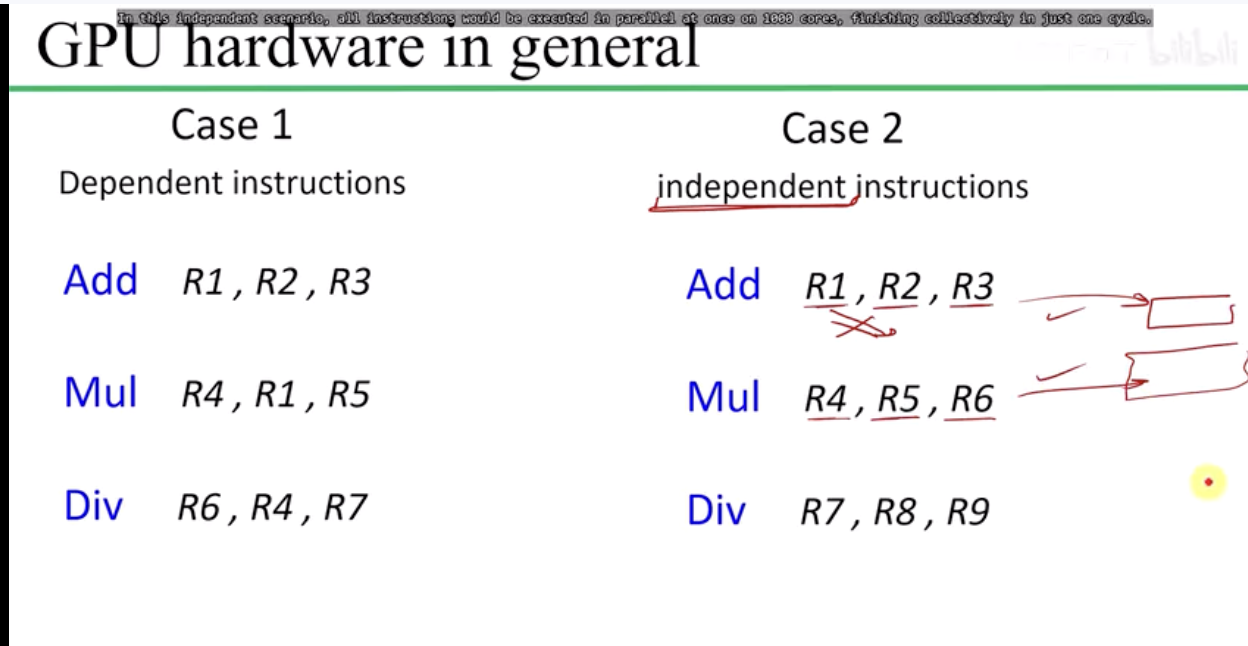
\includegraphics[width=0.75\linewidth]{resources/cuda-003.png}
    \caption{两种计算场景}
    \label{fig:placeholder}
\end{figure}

\subsection{顺序执行与并行执行}

我们将研究两种场景。在第一种场景中，假设大多数应用程序指令是相互依赖的——每条指令都依赖于前一条指令的结果。为此，我们
来看三条指令，每条执行不同的操作：第一条将两个值相加，第二条将它们相乘，最后一条进行除法运算。具体来说，第一条指令从
寄存器 R2 和 R3 中取值相加，并将结果存储在 R1 中。

接着将 R1 中的值与 R5 相乘，将结果存储到 R4 中。这里的关键是这些指令之间的相互依赖性：第二条指令使用了 R1，这个寄存器
正是前一条加法指令的目标寄存器。这意味着在执行乘法之前，加法操作必须先完成。

第二条指令依赖于第一条的结果。同样，除法操作必须等待乘法操作的结果，因为它涉及 R4，而乘法结果就存储在那里。这种处理方式
被称为顺序执行——指令以串行方式一条接一条地执行。你可能会想：为什么不利用多个核心来并行执行这些指令，一步完成呢？在这个
例子中，我们需要三步来执行这三条指令。即使有三个独立的核心分别处理加法、乘法和除法，它们也无法同时运行——第二条指令仍需
等待第一条，第三条等待第二条。

这引出了一个问题：在这种场景下，CPU中少量的ALU反而是理想的选择。如果CPU最适合此类任务，那么我们何时需要GPU？答
案在于指令的性质。虽然我们讨论的场景最适合CPU，但GPU在应用程序内指令相互独立的情况下表现得最为出色。为了说明这一点，
我们来看另一个例子——这次使用相同的加法、乘法和除法指令，但改为每条指令相互独立。

指令之间是独立的，因此如果我们有多个可用核心，就可以将每条指令分配给一个独立的核心，同时并行执行它们。这还可以大规模地发生
。在相互独立的情况下，1000条指令可以在1000个核心上并行执行，总共只需一个周期即可完成。例如，假设我们有1000条指令，
每条执行只需一个周期。而在相互依赖的情况下，将需要1000个周期，因为每条指令必须等待前一条指令完成。

从以上讨论中我们可以推断出：CPU 是专门为顺序操作设计的；而当处理充满大量独立指令的任务时，GPU则处于领先地位——因为
它们能够跨多个核心同时运行多条指令。这里的"顺序"指的是每条指令都依赖于前一条指令的结果。

\subsection{硬件架构}

有一种常见的误解是 GPU 在所有情况下都比 CPU 更好，但这并非事实。接下来我们看看 CPU 和 GPU 在大多数系统中是如何共存的
。下图展示了大多数电脑中的通用主板。你可以看到 CPU 插槽旁装有风扇，专门用于保持 CPU 冷却、防止过热。

主板上还有 DRAM 插槽、电源接口，以及关键的外围组件互连（PCIe）接口。将 GPU 插入 PCIe 插槽后，它就通过主板总线与
CPU 建立了直接连接。PCIe 接口至关重要，因为它允许连接多种扩展卡，包括 GPU、网卡和声卡。当我们把 GPU 插入 PCIe 插槽
时，它就与 CPU 连接起来了。下图展示了 CPU 与 GPU 之间的这种典型连接方式。


\begin{figure}
    \centering
    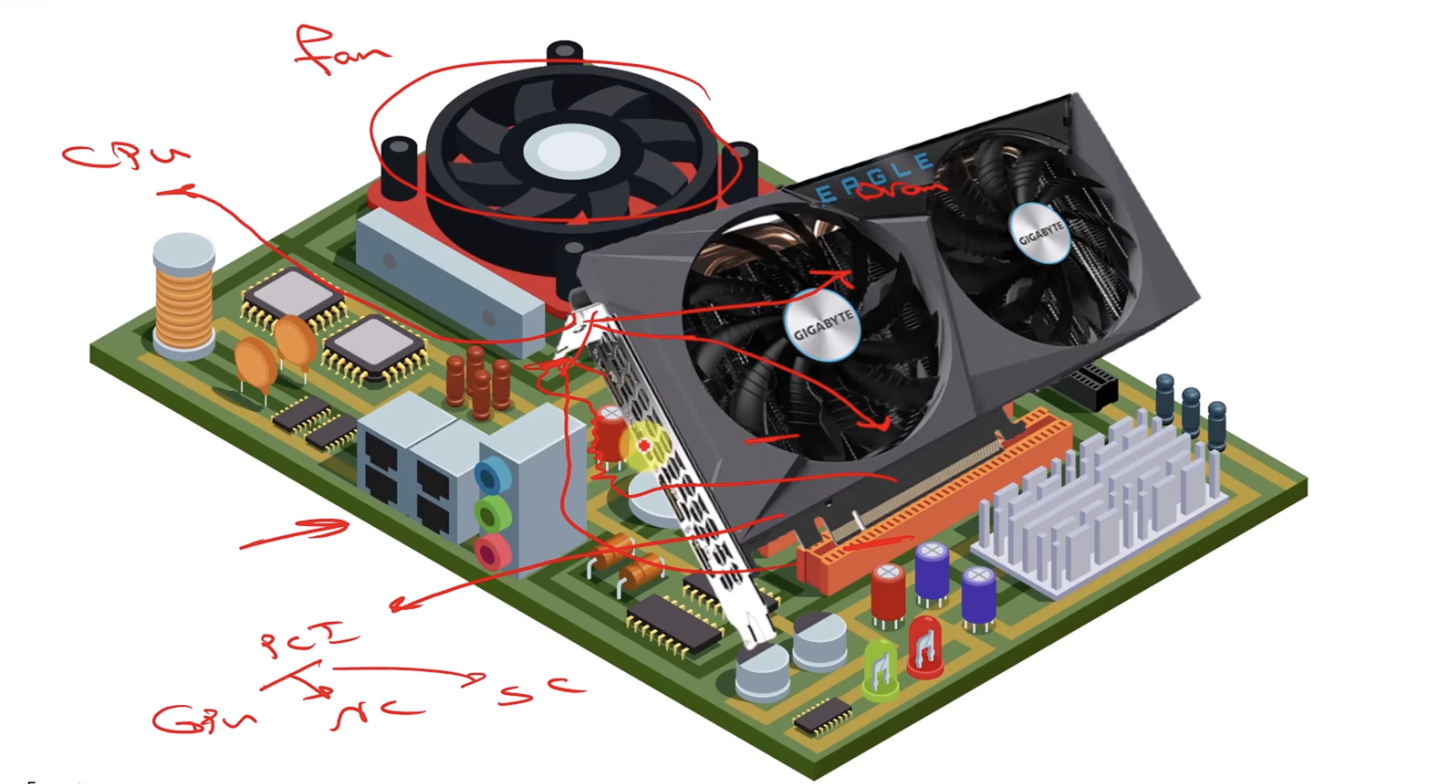
\includegraphics[width=0.75\linewidth]{resources/cuda-002.png}
    \caption{硬件架构}
    \label{fig:placeholder}
\end{figure}

同样，GPU 也有其专用的全局内存。回顾上图，CPU 的全局内存（DRAM）位于内存插槽中，通过总线直接连接到 CPU。

而 GPU 的全局内存则集成在 GPU 扩展卡本身的电路板上。图中绿色方框代表的就是 GPU 扩展卡。本课程的目标正是从最基础的知识
开始，清晰地讲解每一个部分。

\subsection{GPU内部组件}

现在让我们深入分析 GPU 中的关键组件，特别聚焦于英伟达的 GPU。在 GPU 内部有一个关键单元，称为流多处理器（Streaming 
Multiprocessor，简称 SM）。这个术语在本课程中将频繁出现，因此从一开始认识到它的重要性至关重要。此外，诸如调度器和分发
器等组件也存在，我们将在后续章节中更深入地探讨。

除了流多处理器之外，GPU 中还存在多种内存级别，例如 L2 缓存和全局内存。深入来看，每个流多处理器配备了多种针对特定任务
设计的核心：其中一些核心专门用于执行浮点运算，另一些则执行整数运算。

\begin{figure}
    \centering
    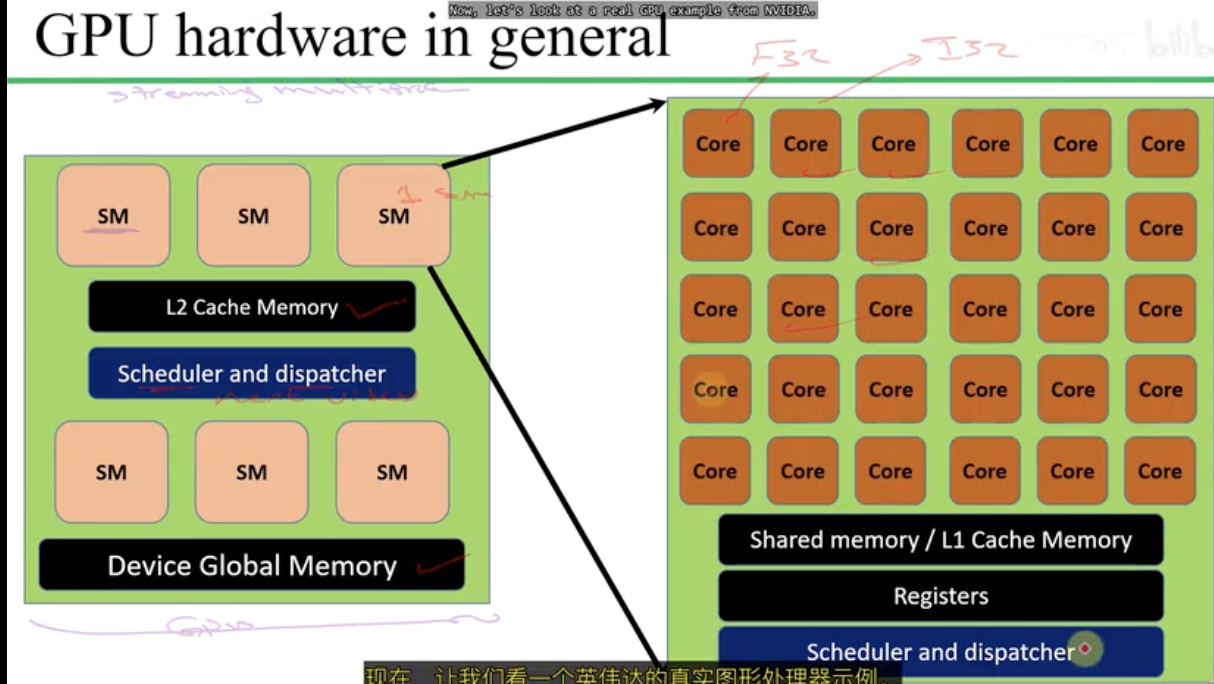
\includegraphics[width=0.75\linewidth]{resources/cuda-004.png}
    \caption{GPU 架构}
    \label{fig:placeholder}
\end{figure}

\subsection{A100 GPU实例}

让我们以英伟达 A100 GPU 为例来看一个真实 GPU 及其流多处理器。A100 于 2020 年发布。下图展示了单个流多处理器的一部分（
并非整个 SM，更不是整个 GPU）。在 SM 内部有 L1 缓存，而 L2 缓存则位于整个 GPU 内部（SM 外部）。需要记住的关键点是
：L1 缓存位于 SM 内部，而 L2 缓存是更广泛的 GPU 层级的组成部分。

\begin{figure}
    \centering
    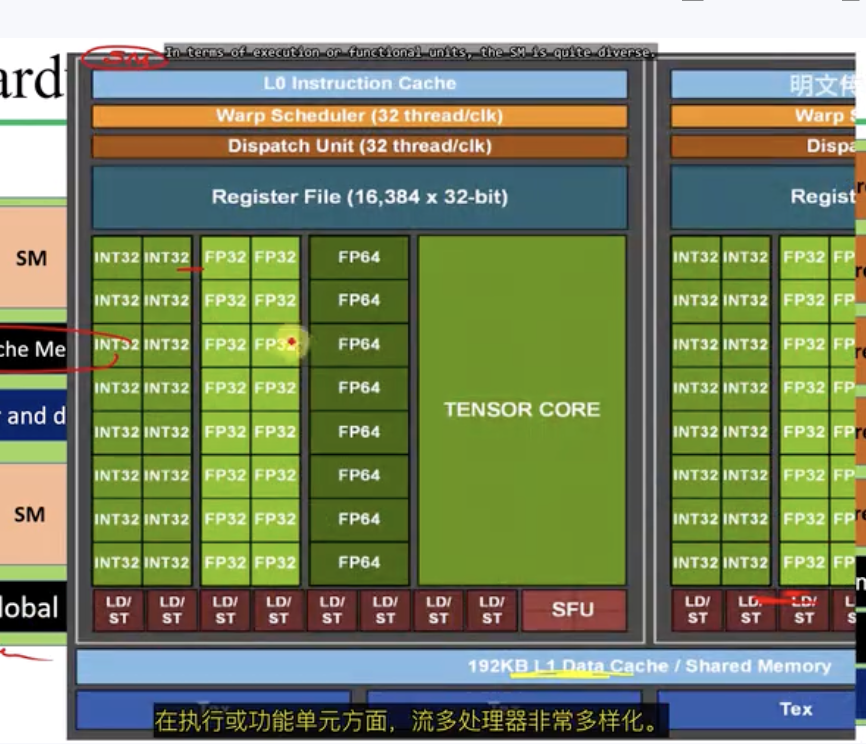
\includegraphics[width=0.75\linewidth]{resources/cuda-005.png}
    \caption{A100 GPU 架构}
    \label{fig:placeholder}
\end{figure}

在执行或功能单元方面，流多处理器非常多样化。我们发现了专门为矩阵乘法操作设计的张量核心（Tensor Core）、用于处理浮点运算
的浮点核心，以及整数核心。此外，如前所述，SM 包含一个调度器单元、一个分发器单元和若干个寄存器。当涉及内存交互时，SM 配
备了加载/存储单元和一些特殊功能单元（SFU）——这些单元负责从内存中读取以及向内存写入数据，并处理诸如对数计算等特定任务。

这张详细的图片仅展示了 GPU 架构白皮书中一个 SM 四分之一部分的快照——这里指的是整个 GPU 的结构图，而非单个 SM。这张
特定的图片详细展示了英伟达 A100 GPU 的规格。在接下来的章节中，我们将更深入地探讨白皮书是什么、在哪里可以访问它们，以
及其他相关细节。

\begin{figure}
    \centering
    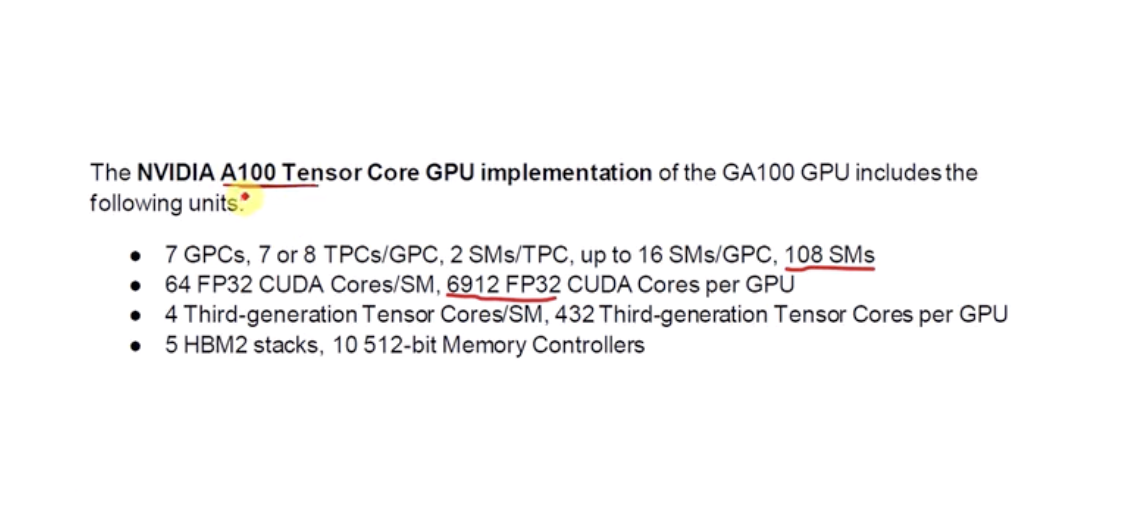
\includegraphics[width=0.75\linewidth]{resources/cuda-006.png}
    \caption{A100 特性}
    \label{fig:placeholder}
\end{figure}


每个 SM 包含 64 个单精度核心。在 A100 GPU 内部，约有 108 个 SM，这意味着整个 A100 GPU 拥有约 7000 个单精度核心——
这是一个非常大的数量。该 GPU 还拥有另外 7000 个专用于整数运算的核心。此外，深入研究 A100 的内部结构，你还会发现特殊功
能单元（SFU）以及张量核心。正是这些核心凭借其庞大的数量所提供的巨大计算能力，使 A100 GPU 成为全球众多高性能超级计算机
的核心组件。例如，META 公司宣布了他们雄心勃勃的计划——建造世界上最强大的超级计算机。如果你查阅 META 官方网站的文章，就会清楚地
看到他们的超级计算机架构严重依赖于 A100 GPU。

在最近的发展中，有推测称他们可能会整合 2022 年发布的新款 H100 GPU——这是在 A100（基于 Ampere 架构）发布两年后推出
的。与 A100 相比，H100 拥有进一步的进步和增强，我们将在本课程中讨论这两者。

你可以在 TOP500 网站
\href{https://top500.org/lists/top500/2023/06/}{https://top500.org} 上找到超级计算机排名列表。
为了强调英伟达 GPU——特别是 A100 GPU——的重要性，让我们看看全球前 500 名超级计算机。该网站提供了关于世界领先超级计
算机的详细信息。从数据中可以看到，A100 GPU 存在于前十名超级计算机中的三台里：它被集成到排名第四的莱昂纳多（Leonardo）超
级计算机中，以及排名第八和第九的超级计算机中。

感谢你与我们一同深入 GPU 的世界，我们下章再见。
